\section{Appendix 3 - Class UML Diagrams}
\label{Appendix_3}

\subsection{Booking and Facilities}
\begin{figure}[H]
    \centering
    \includegraphics[width=0.7\textwidth]{Images/class_uml/booking_facilities.png}
    \caption{UML Diagram of Classes within the \textit{Booking and Facilities} microservice}
    \label{fig:class_uml:booking-facilities}
\end{figure}

\subsection{Challenges}
\begin{figure}[H]
    \centering
    \includegraphics[width=0.8\textwidth]{Images/class_uml/challenges.png}
    \caption{UML Diagram of Classes within the \textit{Challenges} microservice}
    \label{fig:class_uml:challenges}
\end{figure}

\subsection{Fitbit Ingest Service}
\begin{figure}[H]
    \centering
    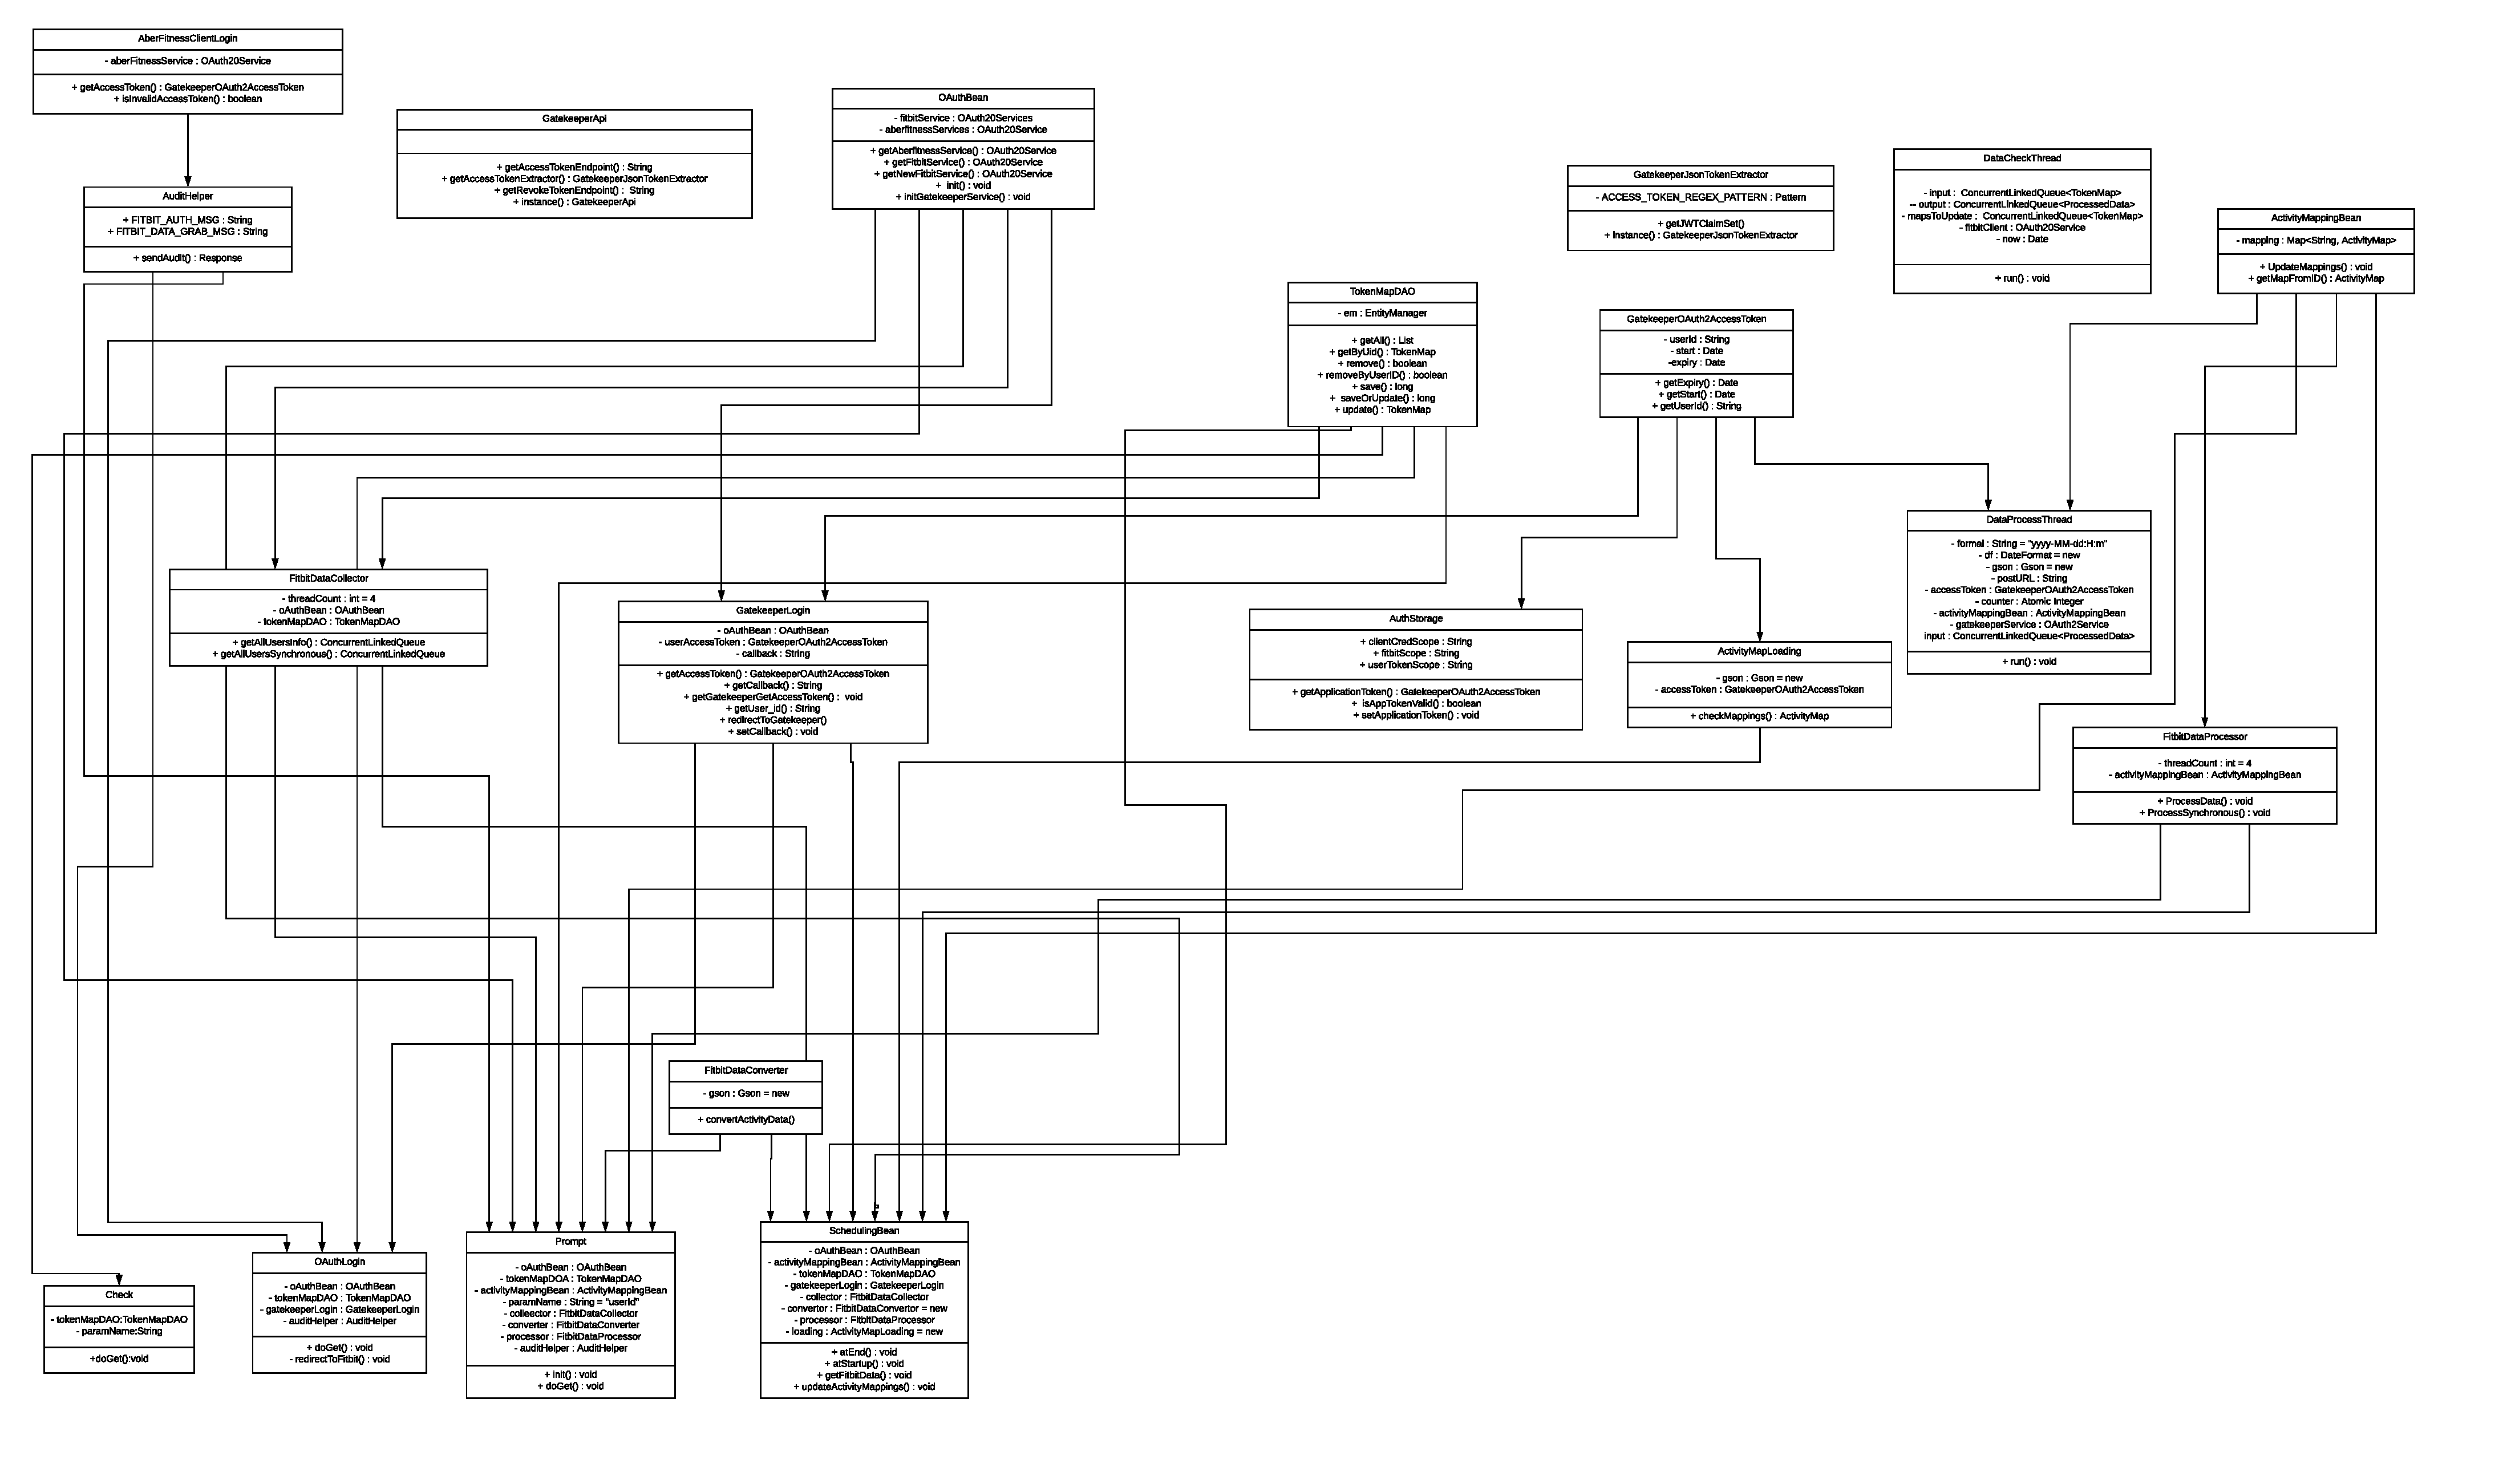
\includegraphics[width=0.4\textwidth]{Images/class_uml/fitbit-ingest-service.png}
    \caption{UML Diagram of Classes within the \textit{Fitbit Ingest Service} microservice}
    \label{fig:class_uml:fitbit-ingest-service}
\end{figure}

\subsection{GLaDOS}
\begin{figure}[H]
    \centering
    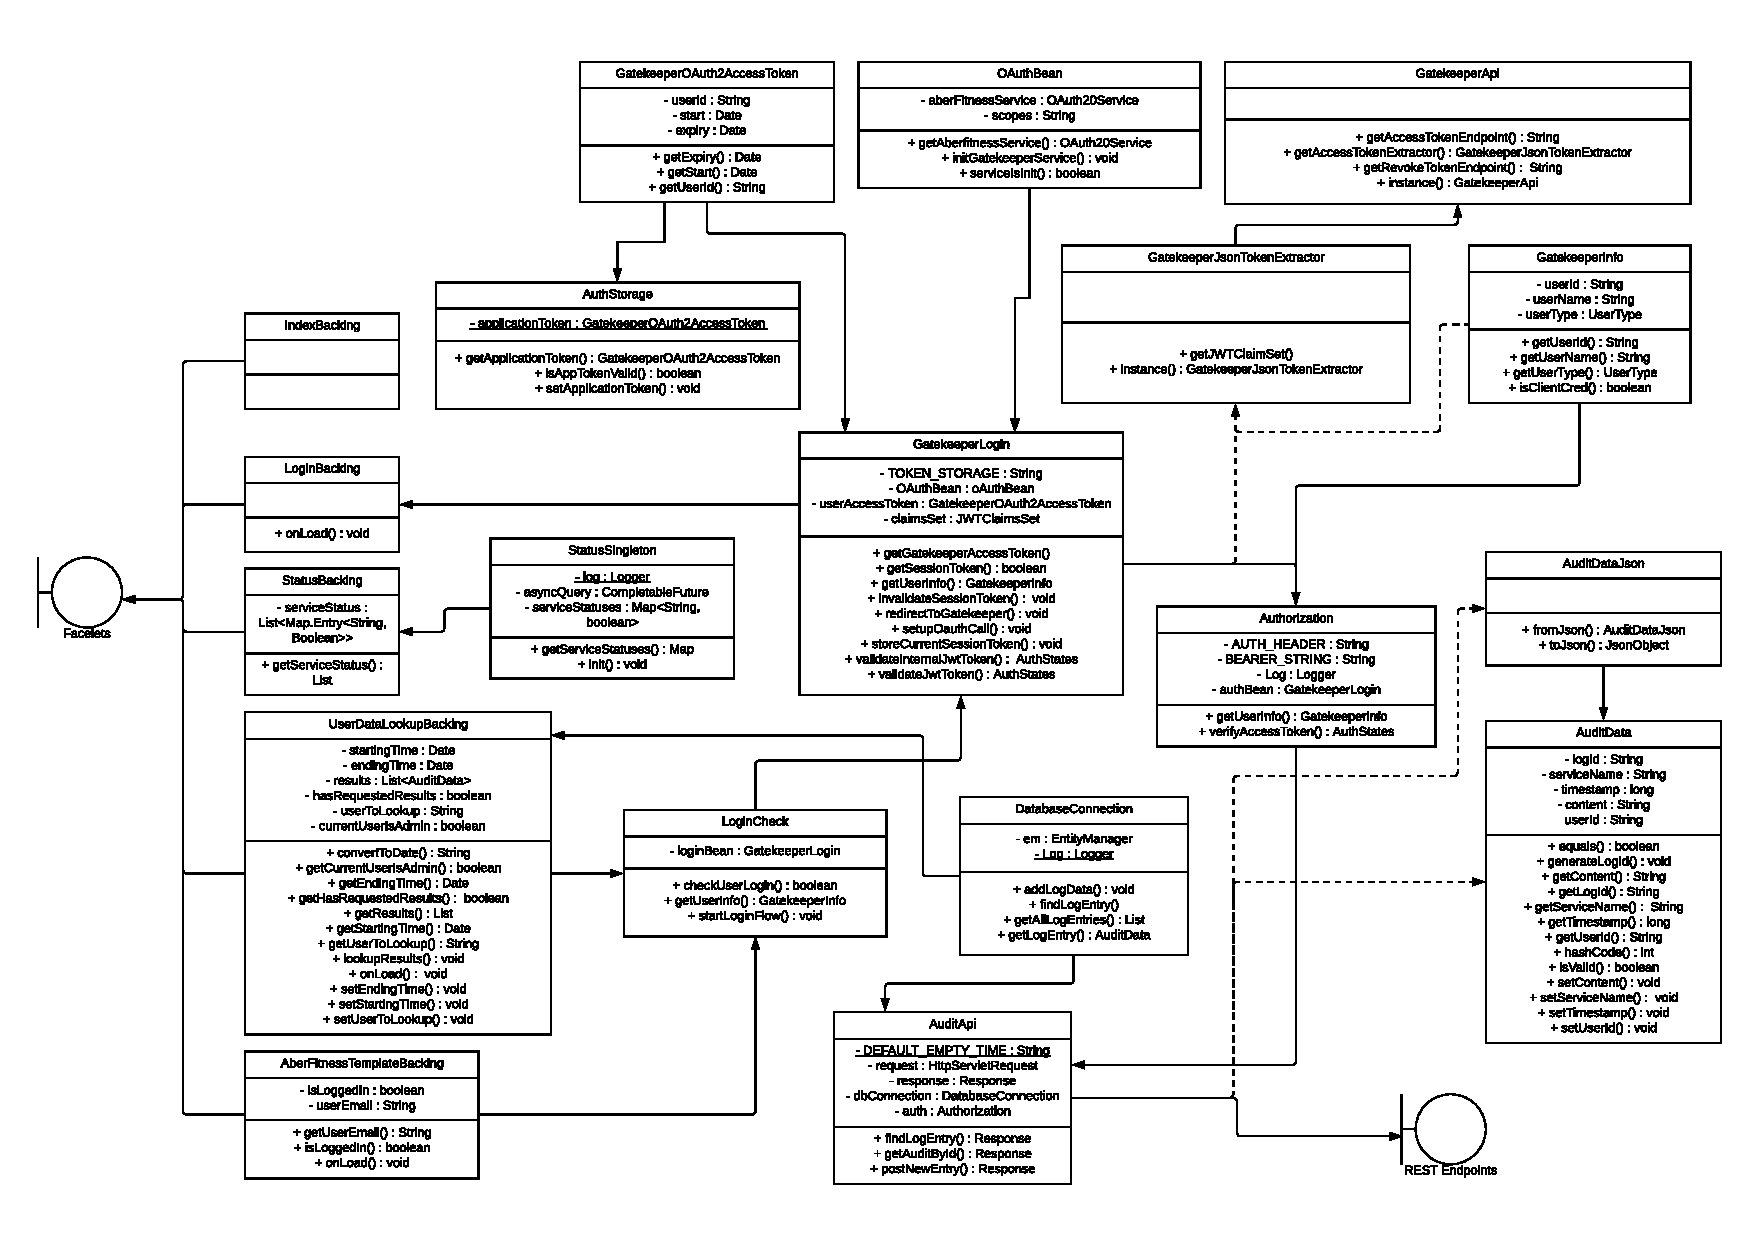
\includegraphics[width=0.3\textwidth]{Images/class_uml/glados.png}
    \caption{UML Diagram of Classes within the \textit{GLaDOS} microservice}
    \label{fig:class_uml:glados}
\end{figure}

\subsection{Ladders}
\begin{figure}[H]
    \centering
    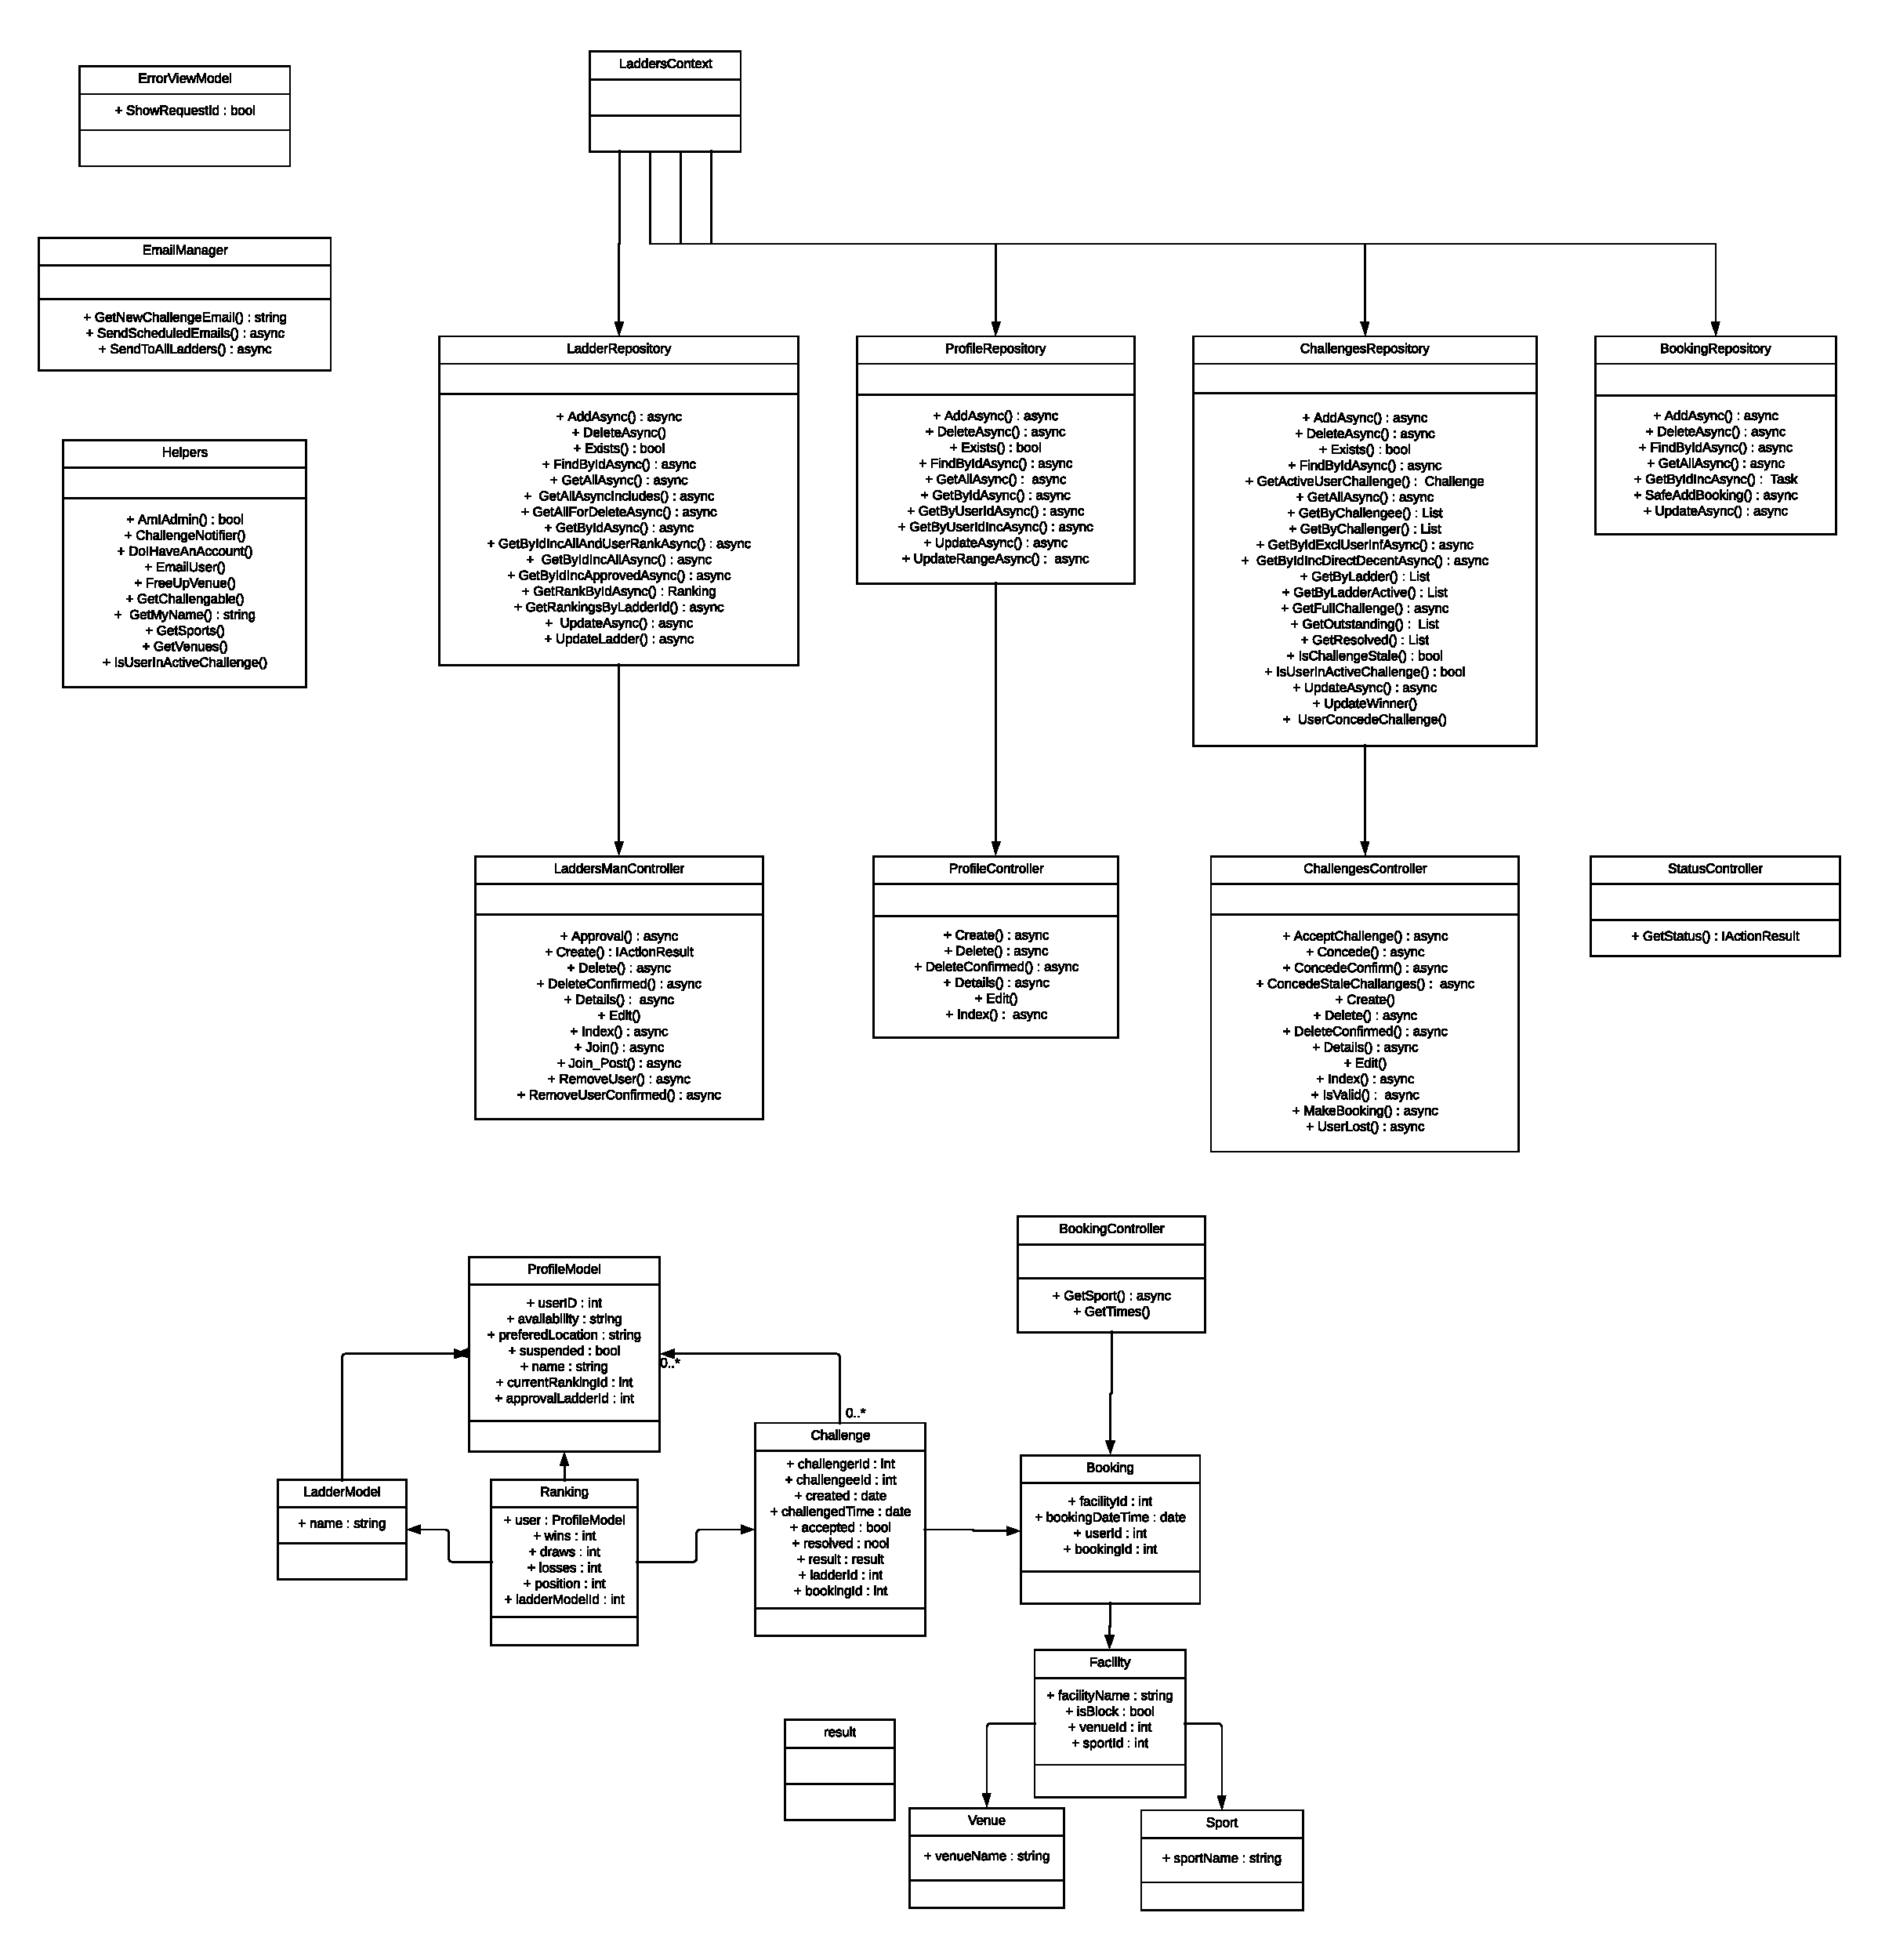
\includegraphics[width=0.7\textwidth]{Images/class_uml/ladders.png}
    \caption{UML Diagram of Classes within the \textit{Ladders} microservice}
    \label{fig:class_uml:ladders}
\end{figure}
